\documentclass[../main.tex]{subfiles}
\begin{document}

\chapter{Docker in Cloud"=Infrastrukturen}
\label{secInfrastructure}
  Wie in der Abschnitt \ref{introVirt} des Grunlagenkapitels gezeigt, bietet der Einsatz von Virtualisierungslösungen, insbesondere Containern, in Rechenzentren einige Vorteile.

  Je nach Anforderungen der Anwendung und der verfügbaren unternehmensinternen Ressourcen und externen Anbieter, lässt sich eine Lösung mithilfe \fig \ref{fig:infrastructure_cloud} und \fig \ref{fig:infrastructure_deployment} bilden.

  \begin{figure}[!h]
      \centering
      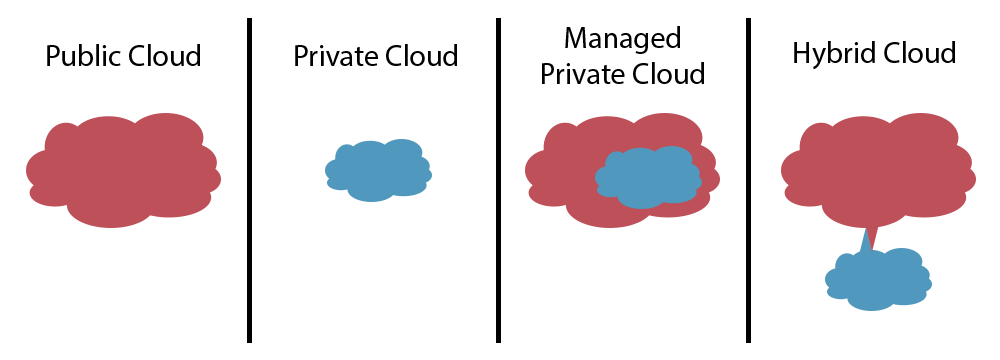
\includegraphics[width=0.9\textwidth]{./images/infrastructure_cloud.png}
      \caption{Verschiedene Arten von Cloud"=Infrastrukturen (eigene Abbildung).}
      \label{fig:infrastructure_cloud}
  \end{figure}
  \clearpage
  \begin{figure}[!h]
      \centering
      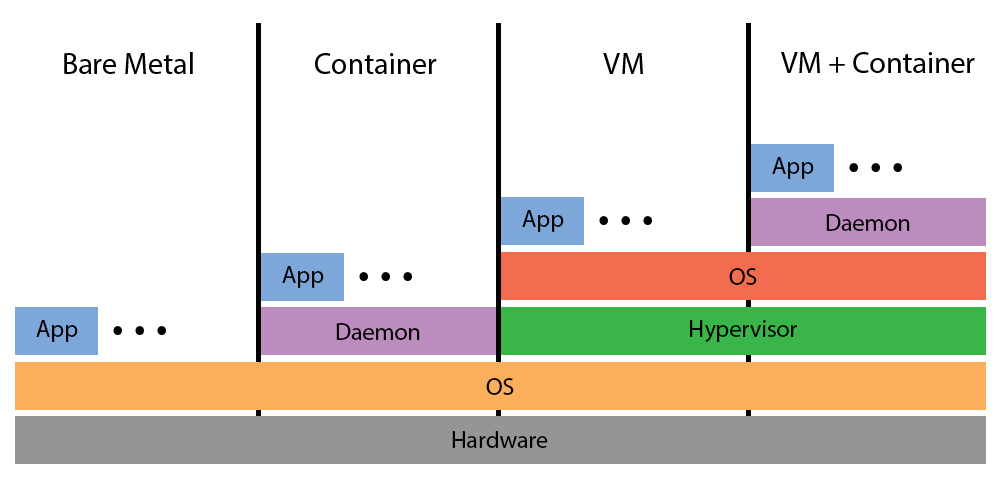
\includegraphics[width=1\textwidth]{./images/infrastructure_deployment.png}
      \caption{Verschiedene Möglichkeiten, um Anwendungen mit und ohne Virtualisierung zu betreiben (eigene Abbildung).}
      \label{fig:infrastructure_deployment}
  \end{figure}

  Exemplarisch sind zwei Situationen aufgeführt, anhand derer Eigenschaften Lösungsvorschläge aus \fig \ref{fig:infrastructure_cloud} und \ref{fig:infrastructure_deployment} konstruiert werden können:

  \begin{enumerate}
    \item Ein großes Unternehmen besitzt die Kompetenz und das Kapital, sichere virtuelle Infrastrukturen zu bauen. Außerdem handelt es sich bei der zu betreibenden Anwendung um eine Software zur Stammdatenverwaltung. Die Anwendung ist daher sehr sicherheitskritisch. \\
    \textbf{Lösungsmöglichkeiten}: Private, Managed Private oder Hybrid Cloud in Kombination mit VMs oder VMs+Container
    \item Ein kleines Startup ohne Investoren baut einen Online-Kartendienst, der als Prototyp frei verfügbar angeboten werden soll. Hohe Sicherheitsanforderungen existieren nicht, da die Anwendung keine Nutzerdaten speichert. Jedoch soll die Anwendung performant laufen. Außerdem sollen für das Startup vielversprechende Entwicklungsstrategien wie \acrshort{CI} und \gls{ImmutableInfrastructure} getestet werden.  \\
    \textbf{Lösungsmöglichkeiten}: Public Cloud in Kombination mit Containern
  \end{enumerate}

  In der Realität sind die Argumentationen weitaus komplexer. Dennoch können bestimmte Lösungsmöglichkeiten in bestimmten Szenarien kategorisch ausgeschlossen werden, während andere attraktiv erscheinen.

  Unabhängig von der gewählten Cloud-Art und Virtualisierungstechnologie lassen sich die Vorteile von Containern bezüglich Automatisierung, \acrshort{CI} und \acrshort{CD} immer nutzen. Auch wenn sich z.\,B. ein Unternehmen aus Sicherheitsgründen für eine Private Cloud in Kombination mit einer hypervisorbasierten Virtualisierung entscheidet, können trotzdem die besagten Vorteile von Containern innerhalb einer VM der Private Cloud genutzt werden, indem in die VMs z.\,B. Docker installiert wird (Architektur \glqq{}VM + Container\grqq{} in \fig \ref{fig:infrastructure_deployment}).

  % Neben der technischen Überlegenheit, hat es Docker durch ein sehr erfolgreiches Marketing geschafft, als Heilmittel vieler Probleme in IT-Abteilungen in Unternehmen geschätzt zu werden.

  % TODO: Was noch Sinn macht, auch in Anspielung auf FRAGESTELLUNG:
  % Grafik (SET 1): "Man hat die Wahl zwischen on premise (private cloud), dedicated hosted in der cloud, und public cloud und mischungen daraus (hybrid cloud)"
  % --> 3-4 Vergleiche bildlich
  % Grafik drunter (SET 2): "Ausserdem hat man die Wahl zwischen VM, Containern, nativ und containern in VM" --> Eine Form von Containern immer gut eigtl wegen Workflow etc.
  % --> 4 Bilder dazu.
  % Aus den Sicherheitsanforderungen der betriebenen Anwendungen/Services kann man aus beiden Sets 2 wählen. Wichtig ist zu checken, ob Auswahl aus Set 2 auch von etwaigen Drittanbietern, die Set1 u.U. beinhaltet, angeboten werden.

  Mit dem CLI-Werkzeug \emph{Docker Machine} stellt \emph{Docker} die Option zur Verfügung, ausgehend von Linux-, Mac- und Windows-Clients lokale und entfernte Docker"=Hostsysteme zu verwalten. Mit frei konfigurierbaren, sowie auf Cloud-Anbietern angepassten Treibern, eignet sich das Werkzeug auch zur Administration von Docker-Installationen in Private und Public Clouds \cite{dockerMachineOverview}\cite{dockerMachineDriverGeneric}\cite{dockerMachineOverviewCloud}.

  Durch den hohen Bekanntheitsgrad und der Popularität von Docker in Ent\-wick\-ler"~ und Managementkreisen sind Anbieter von Public Clouds gezwungen, eine Unterstützung von Docker in ihr eigenes Portfolio aufzunehmen. Tatsächlich reagieren die großen Anbieter wie \emph{Amazon}, \emph{Microsoft}, \emph{IBM} und \emph{Google} mit vielseitigen, häufig Docker-basierten Containerangeboten. Die etablierten Cloud"=Ausprägungen SaaS, PaaS und IaaS werden durch explizite Containerangebote ergänzt, sodass zur Zeit der Begriff CaaS (Container as a Service) als weitere Form von Cloud-Angeboten Gestalt annimmt. Die Auswirkungen von Docker auf genannte Anbieter sind in Abschnitt \ref{publicCloud} beschrieben.

  Auch in Private Clouds ist Docker ein Thema. Die in Kapitel \ref{secLinux} und \ref{secEcosystem} aufgeführten Eigenschaften von Docker eignen sich für eine unternehmensinterne Anwendung der Technologie, wie in Abschnitt \ref{privateCloud} näher erläutert wird.

  %Google: Google Container Engine mit Docker Containern. Mit Kubernetes-Schicht dabei. --> komplette FOSS infrastruktur bei google
  %Amazon: Elastic Bean Stack (fuer web applications) und auch EC2-Container als EC2-Container-Service (ECS)

  \section{Public Cloud}
  \label{publicCloud}
    Während der Begriff CaaS von Unternehmen hauptsächlich für Marketingzwecke genutzt wird, sind sich selbst die großen Vertreter auf dem Virtualisierungsmarkt nicht über die Bedeutung des Begriffs einig. \emph{Google} z.\,B. versteht nach Aussage von Brendan Burns darunter eine Mischform aus PaaS und IaaS, die von ihrer eigenen Entwicklung \emph{Kubernetes} ermöglicht wird \cite[S.12]{slideshareContainerKubernetes}.
    % TODO: Kann man hier sagen "nach Aussage von Google"? Weil die Aussage eigtl. von Vortrag von Brendan Burns kommt, also einem Google-Mitarbeiter.
    \emph{Docker} hingegen umschreibt bei der eigenen Definition von CaaS das Konzept von DevOps, das einen von Docker ermöglichten, flexiblen Workflow der Zukunft realisiert. \glqq{}Der Weg zu CaaS ist mit Docker gepflastert\grqq{} ist eine Aussage eines Artikels des offiziellen Docker-Blogs \cite{dockerCAAS}.

    So versuchen Unternehmen dem Begriff CaaS nach eigenen Vorstellungen Gestalt zu verleihen und ihn zum eigenen Vorteil zu nutzen.

    Fest steht, dass Docker als disruptive Technologie von allen Anbietern von Public Clouds akzeptiert und unterstützt werden muss. Diese Tatsache beruht weniger auf der technischen Überlegenheit von Docker gegenüber anderen Containerlösungen oder der hypervisorbasierten Virtualisierung, sondern auf einem einfachen, automatisierbaren Workflow, der im Modell von \emph{Continuous Integration} und \emph{Continuous Delivery} von Docker ermöglicht wird. Die Innovation, mit der sich IT-Unternehmen aktuell konfrontiert sehen, geschieht dadurch vorrangig auf Prozess- und Geschäftsebene.

    Wie große Public Cloud-Anbieter Docker in ihr bestehendes Produktportfolio integrieren und welche Sicherheitsfeatures diese anbieten, ist am Beispiel von \emph{Azure} von \emph{Microsoft} und \emph{SoftLayer} von \emph{IBM} in den nächsten Abschnitten aufgezeigt. Beide Parteien werben mit einer engen \emph{Docker}-Partnerschaft und guten Integrationsmöglichkeiten von Docker in die eigene Infrastruktur \cite{dockerPartnershipMicrosoft}\cite{dockerPartnershipIBM}. Für beide Produkte stellt \emph{Docker} eigene Treiber zur Verfügung, die von der \emph{Docker Machine} eingebunden werden können \cite{dockerMachineDriverAzure}\cite{dockerMachineDriverSoftlayer}. Die Treiber enthalten Daten wie z.\,B. eine Kundennummer, Anmeldeinformationen und andere plattformspezifische Einstellungen der Public Cloud.

    \subsection{Beispiel: \emph{Microsoft Azure}}
    \label{azure}
      Die Public Cloud-Plattform \emph{Azure} bietet eine Integration von Docker auf Basis von VM-Erweiterungen an. Eine Erweiterung mit dem Namen \emph{Docker Extension} installiert bei der Erstellung einer neuen VM in dieser einen Docker-Daemon. Das Gastbetriebssystem in der VM wird dadurch zu einem Docker"=Hostsystem. Angeblich unterstützt \emph{Azure} aktuell nur die Linux-Distribution \emph{Ubuntu} in der Version 14.04 \acrshort{LTS}. Laut neueren Informationen aus dem Repository der Docker-Erweiterung, wird neben Ubuntu auch \emph{CoreOS}, \emph{CentOS} 7.1 und höher, sowie \emph{\acrshort{RHEL}} 7.1 und höher unterstützt \cite{githubAzureVMExtension}.

      % TODO: Referenz zu Grafik mit 3 Anzaetzen (nativ, container in VM, nur vm)

      Die Docker-Erweiterung lässt sich sowohl über eine Webanwendung als auch über ein CLI-Tool installieren. Auch Zertifikate zur Sicherung der Kommunikation (s. Abschnitt \ref{conClientServer}) können bei der Einrichtung ausgewählt werden \cite{azureDockerExtension}\cite{azureDockerExtensionCLI}.

      Unter \emph{Azure} kann Docker ausschließlich innerhalb einer VM betrieben werden. Grund hierfür ist, dass \emph{Mircosoft} sein eigenes Betriebssystem \emph{Windows Server} sowie seinen eigenen Hypervisor \emph{Hyper-V} nutzt, um VMs zu realisieren. Eine direkte Installation von Docker auf diesem Betriebssystem ist ausgeschlosen, da Docker aktuell nur in Kombination mit einem Linux-Betriebssystem läuft.

      Diese Einschränkung soll mit der nächsten Version des Serverbetriebssystems von \emph{Microsoft}, \emph{Windows Server 2016}, aufgehoben werden. \emph{Windows Server 2016}, das aktuell als Technical Preview 4 vorliegt, verspricht Docker nativ, ohne die Hilfe eines Hypervisors, zu unterstützen. Der Betrieb von Containern auf der Plattform \emph{Azure} wird bereits in den Ausprägungen \emph{Windows Server Containers} und \emph{Hyper-V Containers} diversifiziert. Ersteres sieht die zukünftige Möglichkeit vor, Docker direkt auf \emph{Windows Server 2016} auszuführen. Letztere meint den Betrieb von Containern innerhalb einer VM, wie er aktuell von \emph{Azure} angeboten wird \cite{dockerPartnershipMicrosoft}\cite{azureWindowsContainers}.

      %Im Vergleich zur Konkurrenz werden \emph{Azure} gute Integrationsmöglichkeiten von Public und Private Clouds auf Basis von \emph{Windows Server} nachgesagt, was \emph{Microsoft} zu einem attraktiven Anbieter von Hybrid Clouds macht \cite{IBMDockerOpenStack}.
      % TODO: Kann man das als Quelle ueberhaupt nehmen? Seeehr gewagte These, aber in wissenschaftlichen Papern steht sowas auch nicht....

      Sicherheitsfeatures von \emph{Azure} können, wie Docker, als Erweiterungen in VMs integriert werden. Diese beinhalten u.\,a. Datenverschlüsselung, Firewalls, Intrusion Detection und Anti-Malware Software. Diese Module können unabhängig von Docker für jede VM aktiviert werden \cite{azureDockerExtensionSecurity}. Da diese Module dadurch keinen Bezug zur Art der Virtualisierung haben und für jede VM unabhängig von Docker aktiviert werden können, sind diese Sicherheitsfeatures an dieser Stelle nur kurz erwähnt.

    \subsection{Beispiel: \emph{IBM SoftLayer}}
    \label{softlayer}
      Zwischen \emph{Docker} und \emph{IBM} existiert eine Partnerschaft, die eine enge Integration von Docker in das Portfolio von \emph{IBM Cloud} mit sich bringt. Während \emph{IBM Cloud} überwiegend PaaS-Angebote, insbesondere \emph{Bluemix}, umfasst, ist \emph{SoftLayer} ein von \emph{IBM} erworbenes Unternehmen, deren Geschäftsmodell auf IaaS beruht \cite{IBMDockerServices}. Nach der Definition von Brendan Burns, die CaaS als Mischform aus PaaS und IaaS beschreibt (s. Abschnitt \ref{publicCloud}), deckt \emph{Bluemix} seit der Einführung von Docker-basierten \emph{IBM Containers} im September 2015 auch CaaS-Angebote ab \cite{IBMContainerLaunch}. Das Portfolio von \emph{IBM Cloud} wird wiederum auf der Infrastruktur von \emph{SoftLayer} betrieben \cite{IBMPartnershipDocker}.

      % TODO:Hieraus bessere Textstruktur mit \paragraph{} machen?
      \emph{SoftLayer} klassifiziert seine IaaS-Angebote in Bare Metal- und virtuelle Server. Erstere beziehen sich auf dedizierte physische Hosts, die Kunden in den Rechenzentren von \emph{SoftLayer} mieten können. Auch wenn dieses Modell als Lösung unter dem Namen Private Cloud verkauft wird \cite{softlayerPrivateCloud}, ist es - nach der gewählten Definition des Begriffs im Glossar - kein Angebot der Cloud, sondern klassisches Hosting von physischen Servern.
      % TODO: Sicherstellen, dass die Definition im Glossar das bestaetigt. Cloud: geteilt zwischen mehreren Kunden/Abteilungen und virtualisiert.
      Mit dem zweitgenannten Angebot sind virtuelle Instanzen gemeint, die unter Verwendung von vier verschiedenen Hypervisorn und neun unterschiedlichen Gastbetriebssystemen erzeugt werden können \cite{softlayerSoftware}. Durch die Natur von IaaS sowie den freien Konfigurationsmöglichkeiten, ist der Betrieb von Docker-Containern unter beiden Varianten realisierbar.

      Wie unter \emph{Azure} werden zusätzlich Sicherheitskomponenten angeboten. Auch \emph{SoftLayer} bietet seinen Kunden die Wahl zwischen einigen, bereits in Abschnitt \ref{azure} aufgelisteten Mechanismen unterschiedlicher Hersteller an \cite{softlayerSoftwareSec}.

      % Containers give developers flexibility to build once and move applications without the need to rewrite or redeploy their code. IBM Containers, based on Docker and built on Bluemix, IBM’s platform-as-a-service, provide a more efficient environment that enables faster integration and access to analytics, big data and security services. Enterprises will now be able to use the combination of IBM, Docker, Cloud Foundry and OpenStack to create a new generation of portable distributed applications.
      %   ^   \cite{https://developer.ibm.com/bluemix/2015/06/22/ibm-containers-on-bluemix/}

      % Bluemix basiert auf Cloud-Fountry

      % ganz gutes Bild und ganz gute Infos
      % https://developer.ibm.com/bluemix/2015/06/19/ibm-containers-a-bluemix-runtime-leveraging-docker-technology/

      % Softlayer setzt innerhalb seiner Infrastruktur auf ein hybrides Modell. Neben virtuellen Servern können Kunden sogenannte Bare Metal Server (dedizierte physikalische Hosts) anmieten. Eine Variante die IBM während der Pulse 2014 mit vielen Vorträgen prominent vermarktet hat und mit Performance Tests gegen Rivalen wie die Amazon Web Services schießt, die bekanntlich nur eine virtuelle Infrastruktur anbieten. Nach Angaben von Softlayer werden die Bare Metal und die virtuellen Server mittels derselben API (1.600 Stück), demselben Portal und eigenem internen Managementsystem provisioniert. Zudem sei Softlayer in der Lage, Bare Metal Server zu 100 Prozent automatisiert innerhalb von zwei bis vier Stunden bereitzustellen. Softlayer selbst unterstützt OpenStack derzeit nur als Installation auf den Bare Metal Servern. Das bedeutet, dass die technologische Infrastruktur unterhalb von Softlayer bisher nicht durch OpenStack ausgetauscht wurde.
      % . ... auch sonst ganz gute Infos
      % http://www.computerwoche.de/a/ibm-setzt-konsequent-auf-die-open-cloud,2555573

      % https://www.docker.com/IBM
      % https://docs.docker.com/v1.9/engine/installation/softlayer/
      % Treiber: https://docs.docker.com/machine/drivers/soft-layer/
      % http://blog.softlayer.com/tag/docker

      % Wird von moovel für car2Go Carsharing Service verwendet (s. startseite softlayer)
      % manches auf Basis von OpenStack (http://www.ibm.com/cloud-computing/de/de/infrastructure/)

      % DockerHub ist von SoftLayer gehostet
      % u.\,a. \cite{http://www.businesscloudnews.com/2014/06/11/ibm-links-up-with-docker-takes-it-to-softlayer/}
      % aber da gibts bestimmt bessere Quellen

      % While many people share images on the public Docker registry, security-minded organizations will want to create a private registry by leveraging SoftLayer object storage. You can create Docker images for a private registry that will store all its information with object storage. Registries are then easy to create and move to new hosts or between data centers.
      % \cite{http://blog.softlayer.com/2015/docker-containerization-software}

      % With this in mind, Docker partnered with IBM to launch their first commercial offering – Docker Trusted Registry with commercially supported Docker Engines – in June of this year with availability in North America only. This offering is now available in Europe for businesses looking for a commercially supported Docker solution.
      % What makes it production ready? In addition to formal support from IBM and Docker, Docker Trusted Registry provides clients with a private registry behind the firewall, security and compliance capabilities to manage access control, and integration with existing directories such as LDAP and Active Directory. It also comes with a user interface for administrators to monitor the health of the registry.
      %\cite{https://developer.ibm.com/bluemix/2015/10/23/ibm-and-docker-bring-production-ready-containers-to-europe/}

      % (http://www-01.ibm.com/common/ssi/ShowDoc.wss?docURL=/common/ssi/rep_ca/1/877/ENUSZP15-0561/index.html&lang=en&request_locale=en)
      % --> SoftLayer Bezug?

      % Docker wird in Bluemix eingesetzt und wird unter dem Namen \emph{IBM Containers} vermarktet, also Bluemix-Service.
      % https://developer.ibm.com/bluemix/2015/09/30/ibm-containers-launch-london/
      % https://developer.ibm.com/bluemix/2015/06/22/ibm-containers-on-bluemix/
      % Setpember 2015

      % Delivered as part of Bluemix, IBM’s open cloud platform for application development, the IBM Containers service will enable enterprises to launch Docker containers directly onto the IBM Cloud on bare metal servers from SoftLayer, an IBM company. By leveraging Docker container technology, this will provide companies an environment that is simpler to manage and offers increased utilization and performance in a more flexible execution model, expanding the types of applications that can be supported on the IBM Cloud.
      %

      %SoftLayer vermarketet Multi Tier Security
      %\cite{http://www.softlayer.com/security}
      %mehrere aus: Intrustion Detection System (IDS), Intrusion Prevention System (IPS), beides kombiniert (IDPS)
      %mehrere aus: Firewalls
      %Anti-Virus
      %Security-Benchmark
      %Two-Factor-Authentication
      %\cite{http://www.softlayer.com/SECURITY-SOFTWARE}

      %Schutz vor DOS, wird von einem NOC-Team aufgezeichnet und "migriert" ... was auch immer das heissen soll, s.u.
      %-- A SoftLayer Network Operations Center (NOC) team monitors network performance and security 24x7. Automated DDoS mitigation controls are in place should a DDoS attack occur.
      %-- SoftLayer can’t stop a customer from being attacked, but it can shield the customer (and any other customers in the same network) from the effects of the attack. If necessary, SoftLayer will remove the target from the public network for periods of time and null-routes incoming connections. Because of SoftLayer’s three-tiered network architecture, a customer would still have access to the targeted system via the private network.
      %-- audit and tracking seitens softlayer fuer alle kunden
      %\cite{http://blog.softlayer.com/2014/softlayer-security-questions-and-answers}

      %-- Delivered as part of Bluemix, IBM’s open cloud platform for application development, the IBM Containers service will enable enterprises to launch Docker containers directly onto the IBM Cloud on bare metal servers from SoftLayer.

      %-- mehr flexibilitaet bei softlayer als bei azure, da sowohl bare metal (gut fuer  such as databases and calculation-intensive applications) als auch virtual server angebote.
      %-- "without the overhead of a hypervisor." (http://www.softlayer.com/press/softlayer%E2%84%A2-introduces-bare-metal-cloud%E2%84%A2)
      %\cite{http://www.softlayer.com/BARE-METAL-SERVERS ... und ein tab weiter}

  \section{Private Cloud}
  \label{privateCloud}
    Private Clouds definieren sich dadurch, dass sie von einem Unternehmen in einem eigenen Rechenzentrum betrieben werden.

    Durch die volle Kontrolle über die Hardware des eigenen Rechenzentrums, ist die Bereitstellung von Cloud-Diensten in beliebiger Granularität möglich. IaaS, PaaS und SaaS können einzeln oder in Kombination in einer Private Cloud betrieben werden. In einer solchen Cloud wird die Multi-Tenant-Umgebung von Public Clouds zu einer Single-Tenant-Umgebung, da per Definition nur Cloud-Dienste des Betreibers selbst existieren.

    Diese wichtige Eigenschaft hat direkte Folgen für die Sicherheit:
    % Evtl. Bullets draus machen. 1. keine Trennung nach Kunden 2. Verfügbarkeit weiterhin wichtig 3. Vertraulichkeit und Integrität weniger 4. Vertraute Anwendungen/Umgebung 5. Keine böswilligen Absichten anderer Instanzen bzw. geringere Gefahr anderer Instanzen
    mehrere Kunden müssen nicht mehr, wie es in Public Clouds der Fall ist, voneinander isoliert werden. Eine Trennung innerhalb der Private Cloud gibt es nur noch nach Anwendungen, die nicht miteinander interferieren sollen.

    Während Sicherheitsmechanismen, um die Verfügbarkeit dieser Anwendungen sicherzustellen, weiterhin wichtig sind, kommt solchen, die die Vertrauchlichkeit und Integrität gewährleisten sollen, tendentiell weniger Bedeutung in Private Clouds als in Public Clouds zu. Diese Schlussfolgerung beruht auf der Annahme, dass Anwendungen der Private Cloud von Natur aus vertrauenswürdiger sind, da sie vollständig beobachtet und kontrolliert werden können, sowie oftmals von eigenen Unternehmensmitarbeitern entwickelt wurden.
    % TODO: Wichtig ist hierbei, dass Private Cloud per Definition im Glossar wirklich unternehmenseigenen Rechenzentren meint, also on-premise, nicht off-premise gehosted bei Drittanbietern.

    Diese Sicherheitsvorteile existieren in diesem Ausmaß nicht in Private Clouds, die in Rechenzentren Dritter betrieben werden. Diese Konstellation wird auch als Managed Private Cloud bezeichnet.

    Wie die Bezeichnung aussagt, werden Managed Private Clouds von externen Anbietern verwaltet. Jedoch bezieht der Kunde hierbei keine mit anderen Kunden geteilte Instanz, sondern erhält eine im Rechenzentrum physisch getrennte, dedizierte Infrastruktur \cite{softlayerPrivateCloud}.

    Das potentiell geringere Sicherheitsrisiko in Private Clouds kann sich auch auf die Art der gewählten Virtualisierungsarchitektur auswirken. Der reine Betrieb von Containern auf einem Docker"=Hostsystem ist ohne die Unterstützung von Hypervisortechnologien, je nach Sicherheitsanforderungen, möglich.

    Private Clouds werden u.\,a. als kommerzielle Produkte angeboten. Beispielsweise verkauft \emph{Microsoft} die Lösung \emph{Windows Azure Pack}, welche auf proprietärer Software von \emph{Microsoft} basiert und in Rechenzentren von Kunden installiert wird. Im Open-Source-Bereich dominiert \emph{OpenStack} als Implementierung für Private und Hybrid Clouds, das nun vorgestellt wird.

    \subsection{Beispiel: \emph{OpenStack}}
      %Private Clouds werden häufig mit der Softwareplattform \emph{OpenStack} in Verbindung gebracht.
      \emph{OpenStack} ist eine Open-Source-Software unter der \emph{Apache 2}-Lizenz, die es erlaubt, Cloud-Angebote nach dem IaaS-Modell zu realisieren. Grundlegende Komponenten, die in einem Rechenzentrum existieren, werden über einige Module angeboten. Beispielsweise wird Rechenkapazität mit Nova, Orchestrierung mit Heat und Speicherkapazität mit Swift und Cinder abgebildet. Die einzelnen Komponenten können über eine Vielzahl an APIs miteinander kommunizieren und erfüllen, meist in Kombination, die jeweiligen Anforderungen an eine IaaS-Lösung.

      Durch die Vielseitigkeit und Größe von \emph{OpenStack}, wird der Technologie eine hohe Komplexität und eine lange Einarbeitungszeit nachgesagt. \emph{SUSE} und andere Linux-Anbieter profitieren von dieser Eigenschaft, indem sie z.\,B. mit \emph{SUSE OpenStack Cloud} eigene \emph{OpenStack}-Lösungen anbieten, die Kunden laut \emph{SUSE} eine einfach realisierbare Private Cloud ermöglicht \cite{SusePrivateCloud}\cite[S.2,4]{golemOpenStack}.

      Das Startup \emph{Platform 9} verspricht \emph{OpenStack}-as-a-Service; ein Angebot, das die Komplexität von \emph{OpenStack} für Kunden verbergen soll \cite{platform9}.

      Trotz der Komplexität integrieren viele Anbieter auf dem Cloud-Markt vermehrt \emph{OpenStack} in ihr Portfolio. Unterstützer von \emph{OpenStack} sind u.\,a. \emph{SUSE}, \emph{Red Hat}, \emph{IBM}, \emph{Oracle} und \emph{Intel} \cite{heiseOpenStack}\cite{IBMDockerOpenStack}. Auch die steigende Nachfrage nach Hybrid Clouds in der Industrie, begünstigt \emph{OpenStack}, wie in Abschnitt \ref{hybridCloud} gezeigt wird.
      % \cite{https://opensource.com/resources/what-is-openstack}.
      % Wird als Zukunft von Cloud-Computing gehandelt.

      Die Entwicklung von \emph{OpenStack} ist mit der Verbesserung bestehender und Erstellung neuer Modulfunktionen sehr aktiv. Anfang 2015 wurde mit \emph{Projekt Magnum} ein weiteres Modul angekündigt, das Docker und \emph{Kubernetes} in \emph{OpenStack} verfügbar macht \cite{openStackMagnum}. Davor war ein Betrieb von Containern nur über den Treiber \emph{Nova-Docker} für das Modul Nova möglich, dessen Funktionsumfang im Zusammenhang mit Containern sehr begrenzt ist \cite{heiseOpenStackContainer}\cite{openStackDocker}.
      Magnum nutzt die bestehenden Funktionen von Nova und Heat, die virtuelle Instanzen verwalten und fügt Schnittstellen hinzu, um mit Docker- und Kubernetes-Installationen innerhalb der virtuellen Instanzen zu kommunizieren \cite{openStackMagnum}.

      %Neben der neuen Integration von Magnum, unterstützt \emph{OpenStack} auch viele Hypervisortechnologien wie z.\,B. \emph{KVM}, \emph{XEN}, \emph{Hyper-V} von \emph{Microsoft} und \emph{vSphere} von \emph{VMware}.

      Auch für \emph{OpenStack} bietet Docker einen eigenen Treiber an \cite{dockerMachineDriverOpenStack}.

      % http://getcloudify.org/2015/12/26/openstack-docker-kubernetes-hybrid-cloud-nfv-orchestration-mano-etsi-cloudify.html
      % http://natishalom.typepad.com/nati_shaloms_blog/2014/11/do-i-need-paas-if-i-use-docker.html

      % Das ist gut. auch für Einleitungskapitel, da 1. phzsischer 2. virtual 3. software defined everything chronologisch erklärt wird
      % http://www.golem.de/news/openstack-viele-brauchen-es-keiner-versteht-es-wir-erklaeren-es-1503-112814-2.html

  \section{Hybrid Cloud}
  \label{hybridCloud}
    Hybrid Clouds bezwecken eine Kombination aus Private und Public Cloud. Beide Arten von Clouds bieten Schnittstellen an, die eine Kommunikation der beiden Arten ermöglicht. Für Benutzer von Cloud-Diensten ist die technische und meist geographische Trennung der beiden Infrastrukturen unsichtbar, da diese im Hintergrund von einer Hybrid Cloud-Lösung verwaltet wird.

    Durch die Verknüpfung von unternehmensinternen und -externen Rechenzentren ist die Kompatibilität zwischen beiden Infrastrukturen von großer Bedeutung. \emph{OpenStack} eignet sich daher auch für dieses Szenario, da Abhängigkeiten zu Hybrid Cloud-Produkten mit kommerziellen Technologien vermieden werden. Durch die zunehmende Akzeptanz von \emph{OpenStack} und dessen Integrationsmöglichkeiten in kommerzielle Produkte wird sowohl die bereits genannte, notwendige Kompatibilität gewährleistet, als auch ein sogenannter \emph{Vendor-Lock-In} vermieden. Durch die Verwendung von \emph{OpenStack} kann einfach zwischen Anbietern gewechselt werden. Außerdem können die Angebote von Hybrid Cloud-Lösungen auf der Basis der zugrundeliegenden Open-Source-Technologie transparent miteinander verglichen werden.

    Mit dem Freiheitsgrad einer von \emph{OpenStack} realisierten IaaS-Lösung lassen sich eine Vielzahl von Betriebssystemen und Virtualisierungstechnologien nutzen. Dadurch ist auch der Betrieb von Containern mit Docker und Kubernetes, insbesondere durch das Modul Magnum, jederzeit möglich.

    % TODO:Trend zu hybrid Cloud erwähnen, und Sicherheitsfolgen. Aber Begriff noch sehr schwammig... fehlt es an konkreten teschnischen Lösungen, oder? Sagt ja eigentlich nur aus, dass public und private Cloud nahtlos ineinander integriert werden... was das aus anwendungssicher auch immer zu bedeuten hat.



  % TODO: Docker in/mit VMs

  % Wichtiges Kapitel für Daimler, mein Chef, Management
  % Kapitel, das erst angegangen wird, wenn min. Kapitel 1 steht (Januar 2016 oder später).

  % ???: Transscript aus Besprechung mit Herr Fahner und Patrick:
  % Welche Security-Features uebernimmt die Cloud, welche muss Docker gewaehrleisten. Was
  % bieten MS Azure/Amazon's AWS/etc fuer Mechanismen an?
  % Welche Möglichkeiten zur sicheren Docker-Integration bieten diese?
  % Wortlaut Patrick: Wie funktionierts bei Azure, wie funktionierts wenn man es
  % selbst implementiert.

  % Hypervisor-basierte Clouds:
  % Amazon Web Services (AWS) nutzt XEN.
  % Terremark, Savvis, Bluelock nutzen ESXi.
  % AT&T, HP, Comcast, Orange nutzen KVM.
  % Microsoft Azure und MS Private Cloud nutzen hauseigenen Hyper-V.
  % Container-basierte CLouds:
  % Google, IBM/Softlayer, Joyent (RECHERCHIEN: welche Containerplatform sie nutzen. Google glaube ich lmctfy)
  % ^  \cite[S.2]{dockerLXCKub}

  % formale Definitionen von "Cloud Computing" ...
  % "bare metal cloud": Zuweisung von rein physikalischen Servern und Setups. Kein Overhead von Hypervisorn oder Containerization.
  % ^  \cite[S.1]{dockerLXCKub}

  % Containeranwedungen (Service Discovery Tools) wie HAProxy, Zookeeper, etcd und Consul können eingehende Verbindungen auf mehrere Webserver-Container verteilen --> flexibel und skalierbar. Komplizierte Anwendungen sind deswegen realisierbar.
  % ^   \cite[S.4]{dockerIntroIEEE}

  % Tools wie Docker Swarm und Kubernetes erlauben es, Docker-basierte Appliaktionsstacks auch auf mehreren physikalischen Hosts zu realisieren.
  % Prototyp \emph{libswarm}, jetzt Docker Swarm.
  % Auch für Skalierung, Autoskalierung und Redundanz sehr gut
  % ^   \cite[S.4]{dockerIntroIEEE}

  % Moegliche Kombinationen von VMs, OS, Container, Anwedungen sind in \cite[S.3]{dockerLXCKub}

  % Evtl. mit in Ausblick mit rein:
  % However, using containers for security isolation might not be a good idea. In an August 2013 blog, 4 one of Docker’s engineers expressed optimism that containers would eventually catch up to VMs from a security standpoint. But in a presentation given in January 2014, 5 the same engineer said that the only way to have real isolation with Docker is to either run one Docker per host, or one Docker per VM. If high security is needed, it might be worth sacrificing the performance of a pure-container deployment by introducing a VM to obtain more tried and true isolation. As with any other technology, you need to know the deployment’s security requirements, and make appropriate decisions.
  % ^   \cite[S.3]{dockerLXCKub}

  % Container + VM: wird "Defense in depth" genannt
  % ^   \cite[S.14]{presContainerDockerSec}
  % ^   \cite[S.33]{presContainerDockerSec} --> Details

  % Geringes Organisationsrisiko, da zuverlässige Rollbacks immer gemacht werden können durch Dockerfiles, COW
  % ^   \cite[S.35]{presContainerDockerSec}

  % Deploying Docker on your infrastructure:
  % --------------------------------------------------
  % Both containers and VMs provide isolated environments for running applications on a shared host but from different technical perspectives and can be successfully used separately or together depending on the needs of the application environment.
  % Virtual machines have a full OS, including its own memory management and virtual device drivers. Isolation is provided at the virtual machine level with resources being emulated for the guest OS, allowing for one or more parallel (and, eventually, different) OS to run on a single host. VMs provide a barrier between application processes and bare-metal systems. The hypervisor denies a VM from executing instructions which could compromise the integrity of the host platform. Protecting the host relies upon providing a safe virtual hardware environment for which to run an OS. This architecture has different implications for host resource utilization, but allows for applications with different OS’s to run on a single host.
  % Docker containers share a single host OS across all of the application containers running on that same host. Isolation is provided on a per application level by the Docker engine. Using containers reduces the overhead used per application because the multiple OS instances are avoided. This makes containers lighter weight, faster and easier to scale up or down and can gain higher density levels than full VMs. This approach is only possible for applications that share a common OS, like Linux is used for distributed applications.
  % Regular VMs function in a way that does not allow them to be efficiently scaled down to the level of running a single application service. A VM can support a relatively rich set of applications but running multiple microservices in a single VM without containers creates conflict issues while running one microservice per VM may not be financially feasible for some organizations. Deploying Docker containers in conjunction with VMs allows an entire group of services to be isolated from each other and then grouped inside of a virtual machine. This approach increases security by introducing two layers, containers and VMs, to the distributed application. Additionally this method employs a more efficient use of resources and can increase the density of containers while decrease the number of VMs required for the defined isolation and security goals.
  % Therefore stronger application isolation can be achieved by combining virtualization and containerization than is cost and resource efficient with virtualization alone. Docker containers pair well with virtualization technologies, by protecting the virtual machine itself, and providing defense-in-depth for the host.

  % Running Containers on BareßMetalÖ
  % Containers provide a layer of protection between the host and its applications, isolating between application and the host. This makes it safer to deploy applications on bare-metal when compared to not using any virtualization or container technology. With containers, many application services can be deployed on a single host enabling organizations to gain higher levels of resource utilization out of their infrastructure.
  % However, bare metal deployment does not provide ring-1 hardware isolation, given that it cannot take full advantage of Intel’s VT-d and VT-x technologies. In this scenario containerization is not a complete replacement of virtualization for host isolation levels.
  % Containerization does provide isolation for running applications on bare-metal, which protects the machine from a large array of threats and is sufficient for a wide range of use cases. Users in the following scenarios may not be good candidates to use VMs and can instead use containers; performance-critical applications running on a single-tenant private cloud, where cross-tenant or cross-application attacks are not as much of a concern; or they are using specialized hardware which cannot be passed through to a VM, or which hardware that offers direct-memory-access, thus nullifying the isolation benefits of virtualization. Many users of GPU computing are in this position.
  % Docker containers running on bare-metal have the same high-level restrictions applied to them as they would if running on virtual machines. In neither case, would a container normally be allowed to modify devices or hardware, either physical or virtual

  % TODO: Aus CONCLUSION:
  % Containers and Virtual Machines (VMs) can be deployed together to provide additional layers of isolation and security for selected services.

  % ^   \cite[S.6+7]{dockerSecIntro}

  % TODO: PaaS Use Case
  % Platform as a Service focuses on providing Language Runtime and Services to developers leaving Infrastructure Provisioning and Management to the underlying Layer. PaaS could use Host OS, VM or Container as hosting Environment for applications. PaaS can be implemented using one of the three scenarios.
  % • Option 1 : Each App runs in an Application level container directly on Host OS where PaaS layer runs
  % • Option 2 : Each App runs in a VM on PaaS : Each App runs in its own VM
  % • Option 3 : Each App runs in a container which shares a common VM or VMs for hosting Apps
  % Option 3 is one of the common implementation choice for most of the PaaS vendors as a combination of the VM and container meets some of the requirements of Isolation, Lifecycle management, fair share of CPU time.

  % Using VMs in PaaS:
  % Paas has an important use for VMs to abstract out the Runtime OS from the underlying hardware. Need for each application to have its own VM is the point of contention. Since containers tend to be much lighter in memory footprint, they are preferred architecture as compared to a VM for each application. VM is are used to host the containers. Other Services in Paas like Authentication, Routing, Cloud Controller, Persistent Storage is still run directly on Virtual Machines.

  % From CONCLUSION:
  % Only few PaaS implementations notably the ones which are open source or are new are using containers as opposed to older ones like GAE, Azure which do not use this concept. Containers have a bright future specially in the PaaS use case provided there is more standardization and abstraction from the underlying kernel and Host OS.

  % mittelmaessiges Bild auf S.2

  %     ^   \cite[S.2+5]{virtVSContainer}



  % TODO: Die Frage muss nicht sein: VMs oder Container. Man kann auch VM UND Container zusammen betreiben
  % ^   \cite[S.33]{presContainerDockerSec}

  % TODO: Datencontainer begünstigen auch das MVC-Pattern, welches nach dem Prinzip \emph{Seperation Of Concerns} die verschiedenen Komponenten
  % Multi-Tier-Architektur
  % Seperation of Concerns...
  % bisschen MVC ...
  % strukturierte Architekturen immer gut, begünstigen Sicherheit und Wartbarkeit ....
  % Verfügbarkeit freut sich auch....

\end{document}
